%!TEX root = ../thesis.tex
\section{FIPA Specifications in JADE} % (fold)
\label{sec:fipa}

% Intro to FIPA in JADE/API
\apiname{} closely follows JADE's architecture regarding the use of protocols and services specified by FIPA. 
%The architecture of the API described in this paper includes multiple concepts proposed by FIPA: the \gls{DF}, the \gls{MTS}, the \gls{AMS}, the \gls{ACL} Message and the Interaction Protocols. The following is a brief description of these concepts and of how JADE uses and implements them.

%\begin{figure}
%	\centering
%	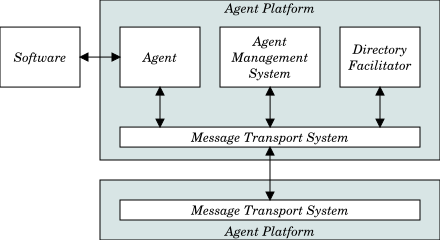
\includegraphics[width=2.5in]{figures/pdf/AMSdiagram.pdf}
%	\caption{
%		Agent Management Reference Model, as specified by FIPA and implemented by JADE. \apiname{} only supports a single Agent Platform.
%	}
%	\label{fig:AMSdiagram}
%\end{figure}

% DF 
The Directory Service (DF) is a component that provides a yellow page service and is part of the FIPA Agent Management Specification. It allows one agent to perform searches about agents rendering specific services. Only agents that are registered in the DF will be indexed and agents can register and deregister themselves at any time.

% DF Agent Description
When searching the DF, agents can use templates that filter the search results. A DF Agent Description represents this template and contains the fields listed in Table \ref{tab:dfAgentDescription}.sim


% MTS
The MTS is a service for transportation of ACL messages between agents. It is responsible for resolving agent addresses, in order to be able to deliver those messages. The MTS may request information from the AMS to perform this address resolution.

% AMS
The AMS is a mandatory component in FIPA-compliant agent platforms. Its purpose is to manage the agent platform, namely the creating and deletion of agents.

% ACL Message
The ACL Message is the envelope that contains the details for communication. The Agent Comunication Language (ACL) stipulates what fields a message should contain. Table \ref{tab:fipaACLMessage} was adapted from the FIPA ACL Message structure specification and contains the list of fields in a message. Not all of them are mandatory. FIPA specifies the \texttt{performative} as the only mandatory field, although the \texttt{sender}, \texttt{receiver} and \texttt{content} are expected to be present.

\begin{table}
	\normalsize
	\caption{FIPA ACL Message Parameters}
	\label{tab:fipaACLMessage}
	\begin{center}
		\fboxsep1pt
		\begin{tabular}{c|c}
		\hline
		\textbf{Parameter} & \textbf{Category of Parameters} \\
		\hline
		\colorbox{Apricot}{\texttt{performative}} & Type of communicative acts \\
		\hline
		\colorbox{Apricot}{\texttt{sender}} & \multirow{3}{*}{Participant in communication} \\
		\cline{1-1}
		\colorbox{Apricot}{\texttt{receiver}} \\
		\cline{1-1}
		\texttt{reply-to}  \\
		\hline
		\colorbox{Apricot}{\texttt{content}} & Content of message \\
		\hline
		\texttt{language} & \multirow{3}{*}{Description of Content} \\
		\cline{1-1}
		\texttt{encoding} \\
		\cline{1-1}
		\colorbox{Apricot}{\texttt{ontology}} \\
		\hline
		\colorbox{Apricot}{\texttt{protocol}} & \multirow{5}{*}{Control of conversation} \\
		\cline{1-1}
		\colorbox{Apricot}{\texttt{conversation-id}} \\
		\cline{1-1}
		\texttt{reply-with} \\
		\cline{1-1}
		\texttt{in-reply-to} \\
		\cline{1-1}
		\colorbox{Apricot}{\texttt{reply-by}} \\
		\hline
		\end{tabular}
	\end{center}
\end{table} 

% Protocols In FIPA
FIPA Interaction Protocols typify communication interactions among agents by specifying two roles: initiator (the agent starting the interaction) and responder (a participant in the interaction). Each protocol defines precisely which messages are sent by each role ad in which sequence.

% Behaviors in JADE
In JADE, every agent activity is programmed through the notion o behaviours. For interaction protocols, typically behaviour-pairs are used for each side of the interaction, and JADE's API supports the most important protocols with built-in initiator and responder behaviours.
% Implementing these protocols.
In order to create an application using these protocols, programmers only need to extend these behaviours and implement the message handlers.
All the complexity regarding the interaction and networking infrastructure is hidden and taken care of by JADE, allowing the programmer to focus on the implementation of agent behaviour.

\subsection{FIPA Interaction Protocols}

To provide a more solid background to the protocols mentioned in this thesis, it's relevant to perform a deeper analysys of them. The two protocols currently supported in the API, as will be explained further ahead in Chapter \ref{chap:solution}, are the FIPA Request, FIPA Query and the FIPA Contract Net. JADE supports a few other protocols, namely FIPA Propose, Iterated FIPA Request and Query and FIPA Subscribe.

\begin{table}
	\normalsize
	\caption{Interaction protocols supported in JADE}
	\label{tab:fipa_protos}
	\begin{center}
		\fboxsep1pt
		\begin{tabular}{c|c|c}
		\hline
		\textbf{Protocol(s)} & \textbf{Initiator class} & \textbf{Initiator class} \\
		\hline
		FIPA request 	& \multirow{2}{*}{AchieveREInitiator} & \multirow{2}{*}{AchieveREResponder}\\
		FIPA Query 		& \\
		\hline
		\multirow{2}{*}{FIPA Contract Net} & \multirow{2}{*}{ContractNetInitiator} & ContractNetResponder \\
		 &  & SSContractNetResponder \\
		\hline
		\end{tabular}
	\end{center}
\end{table}


In JADE, the AchieveRE protocol encompases the multiple ``request-like'' behaviours such as FIPA-Request. It is a simple protocol with three moments of interaction, as Figure \ref{fig:FIPA_request_proto} shows: a request, a response of acceptance or refusal and a facultative result notification. JADE allows the use of other interaction protocols with the AchieveRE: FIPA-query, FIPA-Request-When, FIPA-recruiting and FIPA-brokering. Interaction using this protocol can be 1:1 or 1:N.

The Contract Net protocol starts with a Call for Proposals (CFP) sent to one or more agents, which can reply with a proposal or with a refusal to propose. The initiator can then accept or reject the proposals. As in FIPA-Request, the final result notification is facultative. The ContractNetResponder class from JADE resets itself after terminating the protocol and stays waiting for new CFPs. JADE provides an alternative responder class called SSContractNetResponder that terminates after a single session (SS stands for single session).

\begin{figure}[ht]
	\centering
    \begin{subfigure}[b]{0.44\textwidth}
		\centering
		\includegraphics[height=4in]{figures/FIPA_request_proto.pdf}
		\caption[FIPA-Request protocol]{FIPA-Request protocol}
		\label{fig:FIPA_request_proto}
    \end{subfigure}%
    \begin{subfigure}[b]{0.54\textwidth}
		\centering
		\includegraphics[height=4in]{figures/FIPA_contnet_proto.pdf}
		\caption[FIPA-Contract-Net protocol]{FIPA-Contract-Net protocol}
		\label{fig:FIPA_contnet_proto}
    \end{subfigure}
    \caption[]{Sequence diagrams for the protocols Contract Net and Request. \\Figures are from the FIPA specifications website \footnote{http://fipa.org/})}
    \label{fig:FIPA_Protocols}
\end{figure}
